\documentclass[a4paper,12pt]{report}
\usepackage[utf8]{inputenc}
\usepackage{titlesec}
\usepackage{hyperref}
\usepackage{listings}
\usepackage[ddmmyyyy]{datetime}
\usepackage{fancyhdr}
\renewcommand{\dateseparator}{.}
\usepackage{color}
\definecolor{lightgray}{rgb}{0.95, 0.95, 0.95}
\definecolor{darkgray}{rgb}{0.4, 0.4, 0.4}
%\definecolor{purple}{rgb}{0.65, 0.12, 0.82}
\definecolor{editorGray}{rgb}{0.95, 0.95, 0.95}
\definecolor{editorOcher}{rgb}{1, 0.5, 0} % #FF7F00 -> rgb(239, 169, 0)
\definecolor{editorGreen}{rgb}{0, 0.5, 0} % #007C00 -> rgb(0, 124, 0)
\definecolor{orange}{rgb}{1,0.45,0.13}		
\definecolor{olive}{rgb}{0.17,0.59,0.20}
\definecolor{brown}{rgb}{0.69,0.31,0.31}
\definecolor{purple}{rgb}{0.38,0.18,0.81}
\definecolor{lightblue}{rgb}{0.1,0.57,0.7}
\definecolor{lightred}{rgb}{1,0.4,0.5}
%\usepackage{upquote}
% CSS
\lstdefinelanguage{CSS}{
  keywords={color,background-image:,margin,padding,font,weight,display,position,top,left,right,bottom,list,style,border,size,white,space,min,width, transition:, transform:, transition-property, transition-duration, transition-timing-function},	
  sensitive=true,
  morecomment=[l]{//},
  morecomment=[s]{/*}{*/},
  morestring=[b]',
  morestring=[b]",
  alsoletter={:},
  alsodigit={-}
}

% JavaScript
\lstdefinelanguage{JavaScript}{
  morekeywords={typeof, new, true, false, catch, function, return, null, catch, switch, var, const, let, if, in, while, do, else, case, break},
  morecomment=[s]{/*}{*/},
  morecomment=[l]//,
  morestring=[b]",
  morestring=[b]'
}

\lstdefinelanguage{HTML5}{
  language=html,
  sensitive=true,	
  alsoletter={<>=-},	
  morecomment=[s]{<!-}{-->},
  tag=[s],
  otherkeywords={
  % General
  >,
  % Standard tags
	<!DOCTYPE,
  </html, <html, <head, <title, </title, <style, </style, <link, </head, <meta, />,
	% body
	</body, <body,
	% Divs
	</div, <div, </div>, 
	% Paragraphs
	</p, <p, </p>,
	% scripts
	</script, <script,
  % More tags...
  <canvas, /canvas>, <svg, <rect, <animateTransform, </rect>, </svg, <video, <source, <iframe, </iframe>, </video>, <image, </image>, <header, </header, <article, </article, <g, </g
  },
  ndkeywords={
  % General
  =,
  % HTML attributes
  charset=, src=, id=, width=, height=, style=, type=, rel=, href=,
  % SVG attributes
  fill=, attributeName=, begin=, dur=, from=, to=, poster=, controls=, x=, y=, repeatCount=, xlink:href=,
  % properties
  margin:, padding:, background-image:, border:, top:, left:, position:, width:, height:, margin-top:, margin-bottom:, font-size:, line-height:,
	% CSS3 properties
  transform:, -moz-transform:, -webkit-transform:,
  animation:, -webkit-animation:,
  transition:,  transition-duration:, transition-property:, transition-timing-function:,
  }
}

\lstdefinestyle{htmlcssjs} {%
  % General design
%  backgroundcolor=\color{editorGray},
  basicstyle={\footnotesize\ttfamily},   
  frame=b,
  % line-numbers
  xleftmargin={0.75cm},
  numbers=left,
  stepnumber=1,
  firstnumber=1,
  numberfirstline=true,	
  % Code design
  identifierstyle=\color{black},
  keywordstyle=\color{blue}\bfseries,
  ndkeywordstyle=\color{editorGreen}\bfseries,
  stringstyle=\color{editorOcher}\ttfamily,
  commentstyle=\color{brown}\ttfamily,
  % Code
  language=HTML5,
  alsolanguage=JavaScript,
  alsodigit={.:;},	
  tabsize=2,
  showtabs=false,
  showspaces=false,
  showstringspaces=false,
  extendedchars=true,
  breaklines=true,
  % German umlauts
  literate=%
  {Ö}{{\"O}}1
  {Ä}{{\"A}}1
  {Ü}{{\"U}}1
  {ß}{{\ss}}1
  {ü}{{\"u}}1
  {ä}{{\"a}}1
  {ö}{{\"o}}1
}

\usepackage{graphicx}
\graphicspath{ {./figs} }

\usepackage{caption}

\titleformat{\chapter}{\normalfont\huge}{\thechapter.}{20pt}{\huge}

\pagestyle{fancy}
\fancyhf{}
\cfoot{\thepage}
\setlength{\headheight}{16pt}

%%% title
\title{Showcase of d3.js and its possibilities in infographics using refugee data of the current Ukraine conflict}

%%% author(s)
\author{Luis Rothenh\"ausler (20202459)}

%%% date
\date{Brandenburg, \today{}}


\begin{document}
    %\maketitle
    \pagenumbering{Roman}
        \setcounter{page}{1}
    \newcommand{\THBTitle}[9]{

  \thispagestyle{empty}
  \vspace*{\stretch{1}}
  {\parindent0cm
  \rule{\linewidth}{.7ex}}
  \begin{flushright}
    \vspace*{\stretch{1}}
    \sffamily\bfseries\Huge
    #1\\
    \vspace*{\stretch{1}}
    \sffamily\bfseries\large
    #2\\
    \vspace*{\stretch{1}}
    \sffamily\bfseries\small
    #3
  \end{flushright}
  \rule{\linewidth}{.7ex}

  \vspace*{\stretch{1}}
  \begin{center}
    
\includegraphics[width=2in]{figs/2015_10_05_THB_FB-IM_Logo_RGB} \\
    \vspace*{\stretch{1}}
    \Large  Bachelorarbeit\\

    \vspace*{\stretch{2}}
   \large Fachbereich Informatik\\
    \large und Medien\\
    \large Technische Hochschule Brandenburg\\
    \vspace*{\stretch{1}}
    \large 1. Betreuerin:  #8 \\[1mm]
    \large 2. Betreuer:  #9 \\[1mm]
    
    \vspace*{\stretch{1}}
    \large Brandenburg, den #7 \\
        \vspace*{\stretch{0.25}}

    Bearbeitungszeit: 07.07.2022 - 01.09.2022 % Die Bearbeitungszeit der Seminar-/ Abschlussarbeit ist hier einzutragen.

  \end{center}
}

\THBTitle
      {d3.js and its potential in data visualization\\
      \large Creating a diagram showcase using ukrainian refugee data}        % Titel der Arbeit
      {Luis Rothenh\"ausler}                        % Vor- und Nachname des Autors
      {20202459}
      
      {Technische Hochschule Brandenburg}  % Name der Fakultaet
      {Brandenburg 2022}                          % Ort und Jahr der Erstellung
      {\today{}}                              % Tag der Abgabe
      {Prof. Julia Schnitzer}               % Name des Erstgutachters
      {Prof. Alexander Peterhänsel}                          % Name des Zweitgutachters
    \newpage
    \thispagestyle{empty}

\large
\begin{flushright}
  Brandenburg, den 15.08.2022
\end{flushright}

\vspace*{50mm}
Ich, {\scshape Luis Rothenhäusler}, Student im Studiengang Informatik der Technischen Hochschule Brandenburg, versichere an Eides statt, dass die vorliegende Abschlussarbeit selbstständig verfasst und nicht mit anderen als den
angegebenen Hilfsmitteln erstellt wurde.

Sie wurde in dieser oder ähnlicher Form noch keiner Prüfungskommission vorgelegt.

\vspace*{50mm}

\begin{flushright}
  {\scshape Luis Rothenhäusler}
\end{flushright}

\normalsize
    % This is the german abstract which is required, for some reason.
\chapter*{Abstract - German} % Chapter with * doesn't number
%Englische Arbeiten brauchen eine Zusammenfassung auf Deutsch. Mal abgesehen davon, dass wenn die Zusammenfassung interessant ist man ohne English eh nicht weiter kommt...

%Die moderne Welt produziert täglich riesige Mengen an Daten. Diese zu verstehen und auszuwerten kann in allen Bereichen Grundlage für Entscheidungen und Entwicklung sein. Da es oft schwierig ist große Datensätze zu überblicken und Schlussfolgerungen daraus zu ziehen, wird Datenvisualisierung genutzt Datensätze begreifbar und überschaubar zu machen. Die Ergebnisse von Datenvisualisierung lassen sich überall im Alltag finden. Zum Beispiel als Diagramme in Zeitungen und Nachrichten, sowie die Darstellung von Arbeitsbläufen und Zusanmenhängen unterschiedlicher Faktoren.

%Es gibt eine vielzahl an Werkzeugen die zur Datenvisualisierung genutzt werden können. Während manche dieser Werkzeuge, wie Excel und SPSS, eine Grafische Oberfläche bieten, nutzen andere, wie R und Matplotlib, einen code basierten Ansatz. Die Entscheidung welches der Werkzeuge für die eigenen Anforderungen am besten geeignet ist, ist jedoch nicht immer einfach. Besonders, da die Möglichkeiten, so wie die Vor- und Nachteile der eizelnen Werkzeuge für jemand ohne vorhandene Erfahrung nicht einfach zu überblicken sind. 

Diese Arbeit gibt einen Einblick, sowie eine Einschätzung eines Codebasierten Werkzeuges zur Datenvisualierung, der d3js JavaScript library. Es werden nicht nur das Potential, sondern auch die Vor- und Nachteile evaluiert. Weiterhin wird eine Einschätzung gegeben, wann der Einsatz dieses Werkzeuges sinnvoll ist. Um diese Einschätzungen treffen zu können, werden einige Diagramme, bezüglich der aktuellen Flüchtlichgssituation, die aufgrund des bewaffneten Ukrainekonfilktes besteht, erstellt. Dafür werden zunächst die nötigen Grundlagen erklärt. Dies umfasst sowohl Daten und Datentypen, als auch Diagramme und deren Aufbau. Abschließend werden die erstellten Diagramme, sowie d3js im Diskussionsteil ausgewertet.

Da d3js in reinem JavaScript implementiert ist, lässt es sich Problemlos mit anderen Frameworks kombinieren. Der Fokus von d3js liegt auf der schnellen und einfachen Manipulation von Elementen im Document Object Model. d3js ist jedoch kein Werkzeug mit dem in wenigen Zeilen Quellcode ganze Diagramme erstellt werden können. Vielmehr müssen sowohl die einzelnen Elemente eines Diagrammes, wie auch deren Position und Aussehen händisch definiert werden. Das ermöglicht ein höchstmaß an Kontrolle über das Aussehen und Verhalten der Diagramme. Es ist jedoch auch Zeitintesiv und erlaubt für die Implementation unübersichtilicher Diagramme. Gepaart mit der hohen initialen Lernkurve, kann die Nutzung von d3js nur in speziellen Fällen, welche die volle Kontrolle über Aussehen und Verhalten von Diagrammen benötigen, empfohlen werden.
    \tableofcontents
    \newpage
    \pagenumbering{arabic}
        \setcounter{page}{1}
    \lhead{\nouppercase{\leftmark}}
    %\pagestyle{headings}
    \chapter{Introduction}
%\textcolor{red}{
%Describe the background of the thesis, why it is important, what do we want to achieve.
%Why is this thesis (Motivation)? What do we want to do? What is the status quo? What benefits will result from this thesis?
%Something about the importance of infographics and comprehendible data.}


The postmodern world produces huge amounts of data every second. Analyzing this data can lead to better-informed decision-making in every sector. Yet the wast amounts of gathered data is often hard to comprehend with the human mind. Data visualization is about finding ways to represent this data in visually appealing and easily comprehendible ways \cite{sadiku2016data}. Doing this quickly, ideally instant, and being always up to date can be crucial. While it is possible to create data visualizations manually, it is common to use computer tools to help in their creation. There are many tools available to help with the creation of diagrams for data visualization. Some of these tools have a graphical-user-interface, like Excel \cite{excel}, while others are code based, like R \cite{r} or the Matplotlib \cite{matplotlib} library for Python. As the requirements for a data visualization project can vary, it is often not easy to decide which tool best suits ones needs. Especially when one is unfamiliar with the tools available and has no prior experience. Yet knowing when to use which tool can be greatly beneficial for all parties involved. Therefore this thesis will be a deep dive into the broad possibilities of one of these code based tools, the 'd3.js'(D3) library for JavaScript. Whilst there is a lot of information and examples on how to use D3, the available information makes use of a variety of code styles and different versions of D3. This makes it hard to properly evaluate the possibilities of D3 as a data visualization tool, without using it.

To evaluate D3 and its possibilities there are three main questions that will be investigated in this thesis. What is the potential of D3 in data visualization? What are the advantages and disadvantages of using D3? When should D3 be used? To be able to evaluate these questions and get a better understanding of D3, a showcase of several different diagrams is created and evaluated throughout this thesis. This showcase is created using and visualizing refugee data of the currently ongoing Ukraine conflict. A live version of the showcase can be found at "\url{https://styxoo.github.io/}".

All the theoretical background necessary to understand and follow along with this thesis is described in chapter 2. Afterwards the implementation of the showcase and the diagrams which are contained, is described in chapter 3. Finally in chapter 4 the results are discussed, before drawing a conclusion in chapter 5.

    \chapter{Basics}\label{sec:basics}
%\textcolor{red}{
%Everything necessary to understand the implementation as well as anything which is done beforehand, will come up here}

In this chapter, all concepts, technologies and required backgrounds for understanding this thesis, as well as the showcase implementation, are explained. First, data and data types are described in section \ref{sec:data}. Second, diagrams, their use and how they are structured are described in section \ref{sec:diagrams}. Last, in section \ref{sec:d3}, D3 as the tool to create diagrams is described and its core concepts explained.


\section{Data}\label{sec:data}
%\textcolor{red}{
%Well talk about data a bit. Where does it come from? How is it structured? What kind of attributes? What even are attributes?}
As data is the main content of each data visualization effort, this section gives an introduction to data and data types. While this section only provides a general introduction to data, the data used in this thesis is evaluated in section \ref{sec:data-sets}.

Since ancient times, humans have recorded data. Recording the ins and outs of available resources and other administrative record-keeping were one of the driving factors behind the conceptualization of writing \cite{senner1991origins}.
With the introduction of computers the amounts of gathered data have grown drastically. Nowadays vast amounts of data are gathered across all aspects of life. According to Statista, the total amount of data created, consumed and stored by 2020 was already at 64.2 zettabytes and is projected to reach about 180 zettabytes by 2025 \cite{statista_2022}.

The vast amounts of data gathered in databases are often hard to comprehend and evaluate with the human mind. They are also unwieldy to present in the often limited space of articles, dashboards or other informative purposes. Therefore data visualization (Figure \ref{fig:data-visualization}) is used to turn these data sets, collections of data points, into diagrams. These diagrams can easily be shown in more limited spaces, as well as allow for a quick general understanding and overview of the provided data.

\begin{figure}
    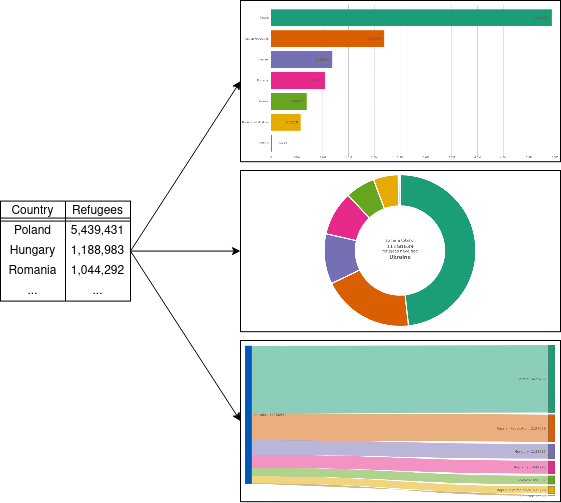
\includegraphics[width=\linewidth]{data-visualization-fin.png}
    \captionsetup{width=0.9\textwidth}
    \caption[data-visualization]{Data visualization describes the process of turning raw data into visual representations. There can be a multitude or possible representations for a data set.}
    \label{fig:data-visualization}
\end{figure}

Data is commonly preprocessed before turning it into diagrams. Depending on the data set and the desired result, this can mean different things. One might want to remove excessive information from the data set, which is not necessary for the representation. On the other hand, additional data can be added by evaluating the existing data points. These could for example be the median of values or grouping of certain value ranges \cite{garcia2015data}. It is important to note, that this preprocessing can happen with specific intentions in mind. While it is only supposed to make the representations easier and more concrete, it can be abused to make data align with the desired results or to create a certain emphasis. This thesis is not too concerned with this, as the possibilities of D3 are independent of the validity and completeness of the presented data.

Even though data comes from a huge variety of sources and can express a plethora of things, there are only four different types of data \cite{henze_2021}. They are split into two categories: categorical and numerical data. Each category has two subtypes. In the following each of the types of data will be explained.

\subsection{Categorical}
%\textcolor{red}{
%What is categorical data? Nominal and ordinal data}

Categorical or qualitative data is information collected in groups. It is often of descriptive nature. Whilst the values can be represented in numbers, like grades, they do not allow for arithmetic operations. Yet as it is possible to count the data points. Therefore it is possible to find the mode. The mode is the most frequently occurring data.

The two sub-types of categorical data are nominal and ordinal data. Each of them is described below.

\paragraph{Nominal}
data is mostly descriptive in nature. Values have no relation to each other and have no inherited order. Examples are the 'Country of origin', 'Color of paint' or 'Brand of car'.

\paragraph{Ordinal}
data is also descriptive, yet the data does have a internal order. For example different dates each describe a day, but one day also comes after another. Grades also have an internal order, as one grade is better then another. Whilst ordinal data has an ordering, the order is not necessarily equidistant. Due to its internal order, it is also possible to find the median. The median is the value where half the values in the data set are higher and the other half of the values are lower.

\subsection{Numeric}
%\textcolor{red}{
%What is numeric data? Continuous and Discrete}

Numeric or quantitative data is all data expressed in numbers, where numbers do not represent categories. It allows for arithmetical operations and can be split into discrete and continuous data.

\paragraph{Discrete}
data can only take certain defined values. This usually means whole numbers to represent things that can not be split up further.  Discrete data is usually countable. Examples are the 'Number of Refugees' or 'Tickets sold'.

\paragraph{Continuous}
data can be measured. It can have any real number as value. Therefore fractions are possible as well. For example when measuring the temperature, or the length or weight of an object.


\section{Diagrams}\label{sec:diagrams}
%\textcolor{red}{
%What diagrams exists? Which are the most common? What possibilities do they offer for encoding data? Which considerations for readability? Why do some diagrams not make as much sense? Which considerations where made for fulfilling the showcase requirements?}
This section first provides a brief introduction to diagrams, containing an overview of the history of diagrams, where they can be found and what their potential is. How diagrams are constructed using marks and channels, as well as what needs to be considered while doing so, is described afterwards.

\subsection{Introduction}
Using graphical representations to convey data has been done by humans since the earliest cave paintings. In the 18th century William Playfair bar and column, as well as pie and donut charts \cite{dur2012analysis}. Since then, diagrams have only become more common. Nowadays one constantly comes across diagrams as the results of data visualization in everyday life. They can be commonly found across all kinds of reports, information campaigns or as part of user-interfaces in machinery or control systems. This is not only due to the fact that diagrams not only allow the representation of a lot of data in limited space. They can also represent the data in a more attractive ways. Additionally, data seen in diagrams is easier to remember, as "The human brain is more able to identify and comprehend relationships and patterns if data is encoded into visual forms."\cite{cleveland1985elements}. This is one of the main reasons that diagrams are used so frequently in newspapers \cite{utt2000update}.

With the frequency of diagrams in use every day, some diagrams are, intentionally or not, inaccurately representing information. Due to the huge potential diagrams offer for the perception of data, this should be carefully considered. Edward Tufte introduced the lie factor for evaluating how accurately data is shown \cite{tufte}. It is defined as the effect size in the diagram over the effect size in the data. Most sources of skewed representations of data can be prevented by using zero baselines, equidistant axes, accurate scaling when using areas and value adjustments for monetary values to contradict inflation influences.

Yet the selection of which diagram should be used to visualize which data set is not trivial. Mostly there are several possible diagram choices for any given data. Furthermore there are a plethora of diagrams already in use and anyone can create totally new diagrams to suit their needs. Yet the vast majority of use cases can be accomplished by one of the more commonly known diagram types, like bar and column charts, pie and donut charts and line charts \cite{lankow2012infographics}. Due to their popularity, tools like Excel provide support for these diagrams out-of-the-box \cite{office_chart_types}. More specialized diagrams might use combinations or variations of other diagram types. Other diagrams are specifically created for only a visualization.


\subsection{Marks and Channels}
Whilst there are countless types of diagrams, most diagrams use a combination of marks and channels to present data. Marks are used for entries in the diagram. The three possible marks are points, lines and areas. Channels describe the way specific marks encode data. While there is no definitive list of channels, the most commonly used channels are position, size, color and texture. The position in 2D can be split into the x and y positions. The color can be split into hue and luminescence. Each mark should use at least one channel to encode data. Otherwise it does not convey any information. For example in fig. \ref{fig:bar-chart} lines are being used as marks for each of the seven entries. It might seem like areas are used. Yet the thickness of the line, and therefore the bar, only serves visual understanding and holds no relevant information. The lines use three channels to encode data. The y-position is used to represent the categorical data of which country. The hue of the bar encodes the same data. This is a bit redundant, as the country is already encoded. Yet the hue makes it easy to follow along when data is changing and bars are shifting positions. The size, in this case length, of the bar encodes the discrete data of how many refugees have crossed into the country. In fig. \ref{fig:marks-area} areas are used as marks. Just like in the previous example the hue encodes the country and the size encodes the refugee count. 

\begin{figure}[ht!]
    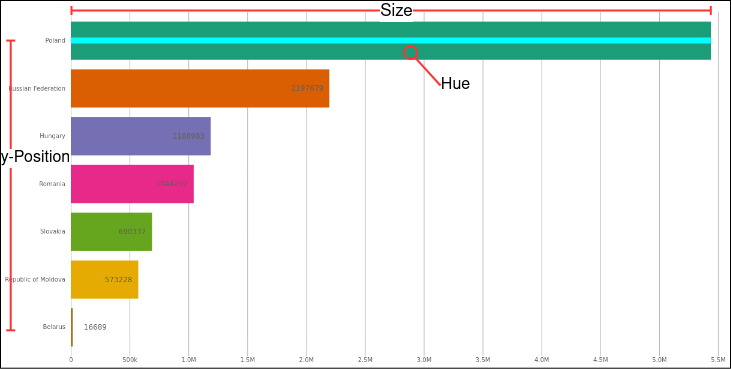
\includegraphics[width=\linewidth]{marks-bar-chart.png}
    \captionsetup{width=0.9\textwidth}
    \caption[bar-chart]{This bar chart uses lines as marks. Each bar is a single line mark. The first line mark is highlighted in cyan. The thickness has no relevance other than making the line visible. Each mark uses three channels to encode data. They are highlighted in red. The y-position and the hue are used to encode the country. The size of the line, aka the length, corresponds to the number of refugees.}
    \label{fig:bar-chart}
\end{figure}

\begin{figure}[ht!]
    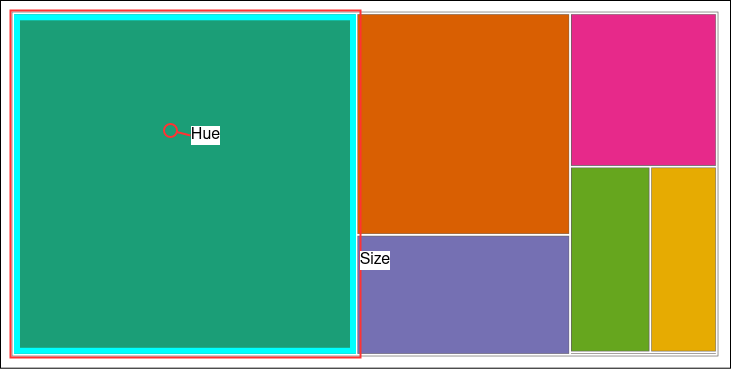
\includegraphics[width=\linewidth]{marks-area.png}
    \captionsetup{width=0.9\textwidth}
    \caption[marks-area]{This tree map uses areas as marks. A representative mark has been highlighted in cyan. The areas use the size and hue channels to encode data. The size corresponds to the number of refugees, while the hue corresponds to the country.}
    \label{fig:marks-area}
\end{figure}

All marks can be used with all channels. But not all data types should be represented by all channels. For example nominal data should not be encoded using the size channel. The different sizes would lead to a perceived order, which does not exist in nominal data. As the channels all differ in their appearance they are also not equally good in adequately representing the data types. Therefore it is important to consider which channels are chosen to represent the given data types. According to a study by Jock Mackinlay from 1986, the position channels can always be considered the strongest channels, no matter which marks are combined with them \cite{mackinlay1986automating}. Therefore the selection of marks and channels should be considered carefully. If chosen poorly it can lead to undermine the purpose of the diagram of easily presenting data to a viewer.

Another factor which plays a role here, is the data-ink ratio described by Tufte \cite{tufte}. It describes the ratio of ink necessary for representing data over the total ink necessary for the diagram. The idea is to draw only what is necessary for showing the data, as this is the main purpose of a diagram. Whilst a lot of diagrams are digital nowadays and therefore do not require ink, diagrams should still try to get as close as possible to a data-ink ratio of one. The lower the data-ink ratio drops, the harder it gets for a viewer to see and comprehend the relevant data.

As some viewers might not be able to perceive the whole range of colors, choosing a color scale should also be carefully considered. Besides using colors which retain a high contrast even with color blindness, they should also be perceptually uniform. This means having similar hues for values close together, and more distinctively different hues for values further apart, but also having a consistent rate of change in the hue. This is especially important when trying to encode quantitative data using the hue channel.


\section{D3.js}\label{sec:d3}
%\textcolor{red}{
%This is all about d3. What is it? Where does it come from? What is it used for? Who uses it? Why should it be used? How does it work? Enter, update and exit pattern. Something about the modular structure of D3 as well. Might be worth mentioning "observables" as well.}

While there are many ways to turn data into diagrams, this thesis makes use of D3 to achieve this. Therefore this chapter introduces D3 by elaborating what it is and how it works.

"D3.js is a JavaScript library for manipulating documents based on data. D3 helps you bring data to life using HTML, SVG, and CSS."\cite{d3js}. The name D3 is short for data-driven documents. The D3 library was originally created by Mike Bostock and is published under the BSD-3-Clause open-source license. It is about 350kB in size. As it is fully implemented in JavaScript, it does not require a specific framework and can therefore be easily integrated into all kinds of web-based projects. Whilst D3 is not limited to using SVG, the visualization created using D3 mostly rely on SVG elements for their implementation.

D3 is not a high-level API for creating out-of-the-box visualizations. Instead, "[it] allows you to bind arbitrary data to a Document Object Model, and then apply data-driven transformations to the document."\cite{d3js}, therefore making Document-Object-Model(DOM) manipulation easier and less tedious. The DOM represents the structure of an HTML in memory and offers scripts the possibility of accessing and modifying the represented HTML. D3 also provides helper functions like scales, to decrease the amount of mathematical equations needed to convert from the data range to the necessary coordinates in the desired visualization.

There are three main concepts that make up the core of D3. Selections, data joins and the general update pattern. All three concepts are working closely together. Whilst selections can be used without data joins and the general update pattern, these two aspects both rely on selections. Data joins can also be used without explicitly using the general update pattern. Usually all three of these concepts are used consecutively. First, a selection is created. This selection is then used to create a data join. Finally, the behaviors of the general update pattern are defined for this data join.
In the following all three of the core concepts of D3, as well as scales and D3's plugins are explained.


\subsection{Selections}
%\textcolor{red}{
%What are they? Why are they useful?}

A selection contains references to one or more DOM elements. These references are organized in groups. There are two functions in D3 to create a new selection: \verb|d3.select("selector")| and \verb|d3.selectAll("selector")|. Both functions require a selector for identifying the appropriate elements. The selectors are defined in the "W3C Selectors API" \cite{w3c_selectors_api} and function like CSS selectors. Whilst \verb|select| only selects a single element, the first element matching the selector, \verb|selectAll| selects all elements which match the selector. It is important to note, that \verb|select| also propagates the existing information of this node, whilst \verb|selectAll| does not. Selections can also be extended or shrunken by adding or removing groups, or by combining multiple selections. \verb|select| and \verb|selectAll| can also be called on on elements of an already existing selections. The selector will then assume the existing element as root for its selection process.

It is possible to directly access DOM elements through the selections. The respective DOM elements are linked in the groups which make up the selection. But usually this is not required, as there are predefined functions for easily modifying properties for all elements referenced in a selection. This includes the modification of attributes and styles of DOM-elements, as well as event handling.

A selection is required before a data join can be made. How this is achieved is described in the following section.


\subsection{Data Joins}
%\textcolor{red}{
%What are they and why are they important?}

\begin{figure}[ht]
    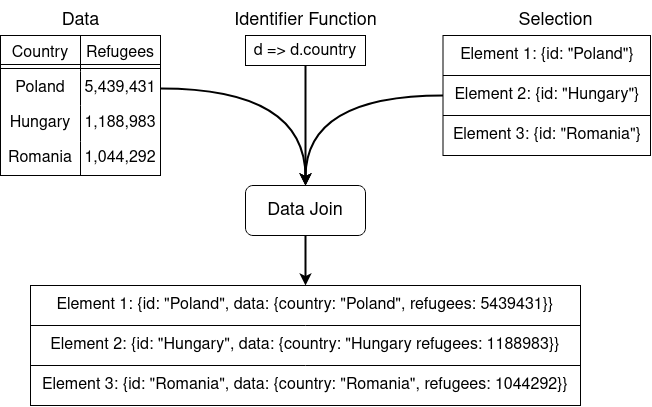
\includegraphics[width=\linewidth]{data-join.png}
    \captionsetup{width=0.9\textwidth}
    \caption[data-joins]{A representation of how data joins are created. A selection, consisting of DOM-elements, as well as the data need to be present first. The data join then combines the two. The identifier function is needed if the diagram is supposed to be able to update and can be specified when creating the data join. As a result the data is matched to the applicable DOM-elements using the identifier function.}
    \label{fig:data-joins}
\end{figure}

Data joins are the second key feature of D3. They bind a specific data point to a specific DOM element. To create a data join, one has to first create a selection of elements. These are the elements one wants to match to specific data points. The data join is then created by calling the \texttt{.data(dataSet)} function on the selection. It takes a data set, an array of objects where each object represents a single data point, as parameter. This will bind the data points to the applicable elements in the selection. This is achieved by using an identifier function. This identifier function is called for each data point in the provided data set. The default identifier function returns the index of the current data point in the data set. When one wants to create diagrams which can respond to data changes over time, this is not a reliable identification. When data points are removed or added in arbitrary locations, the index will not match the elements it previously did. Therefore a custom identifier function can be specified, as seen in figure \ref{fig:data-joins}. This can be passed as the optional second parameter of the data function, will be called for each data point and has to return some value which will be used as the ID. This ID is saved on the element the data point was matched to. Every time the data set is updated, the data join and its underlying selection need to be called again.

As seen in fig \ref{fig:general-update-pattern}, it can be that the number of data points does not match up with the number of elements to represent them. When there is no element matched to a certain data point, D3 will create an empty placeholder node for this data point. What happens to the placeholders is defined in the general update pattern.


\subsection{General Update Pattern}

\begin{figure}
    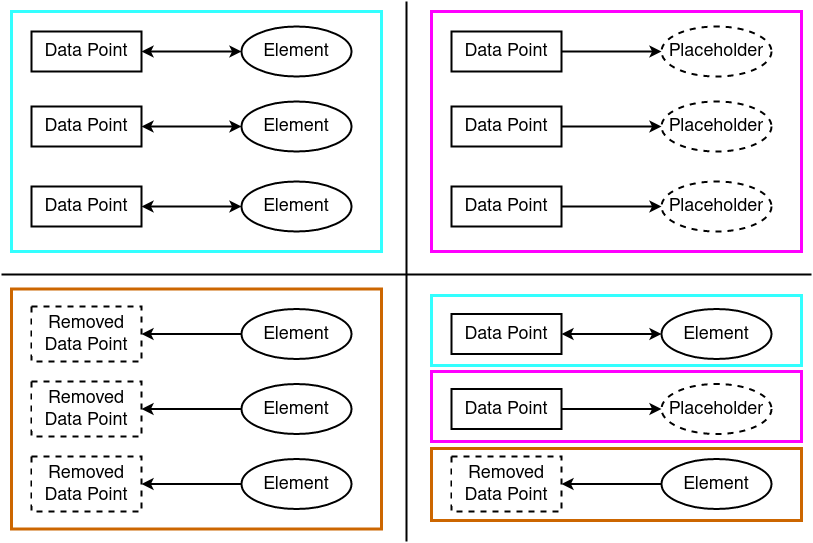
\includegraphics[width=\linewidth]{data-joins-fin.png}
    \captionsetup{width=0.9\textwidth}
    \caption[general-update-pattern]{A representation of the possible cases when creating data joins. In the top left, the data join was able to match all data points to an element of the provided selection. Those cases are marked in cyan. In the top right, there are data points but no elements in the provided selection. Therefore they are matched to placeholder elements. These cases are marked in magenta. In the bottom left, the provided selection is filled with elements, but their previously matched data points have been removed. These cases are marked in orange. The bottom right shows that all three previous cases can exist in a single data join. For each of the three cases, the general update pattern can have different behavior specified.}
    \label{fig:general-update-pattern}
\end{figure}

The general update pattern is another core concept of D3. Every time a data join is created or updated, it can be made use of. The general update pattern differentiates between three different cases: enter, update and exit. For each of these cases a sub-selection is created by the data join. For each of these three sub-selections the behavior can be defined. As sub-selections are just selections themselves, they will be referred to as such henceforth. The first selection is the enter selection. It corresponds to the magenta elements in fig \ref{fig:general-update-pattern}. All the placeholders created by the data join for data points without a matching element are in here. In the behavior for the enter selection, usually a corresponding element is created as the first step. Often these elements serve as the marks representing data points in the diagram. Adding elements includes providing enough attributes to the elements, for them to be appropriately matched the next time the data join is called. When creating an element which is a mark in a diagram, providing appropriate attributes and styles of an element which corresponds to using the desired channels for data encoding.

All the elements which are already linked to a data point and therefore identified correctly using the identifier function, make up the update selection. They are marked in blue in fig \ref{fig:general-update-pattern}. Specifying the behavior of the update selection allows the diagram to react to changing data by moving existing elements or changing their appearance to accommodate for other new or removed elements.

The last selection, the exit selection, is made up of all the elements previously matched to a data point, for which the corresponding data point has been removed from the data set. They are marked in orange in fig \ref{fig:general-update-pattern}. The behavior of the exit selection is by default defined to remove the respective elements. The exit behavior can be defined if a more visually pleasing removal of elements is desired, like fading out before deleting.

When the goal is to create only static diagrams, which are only initially created from data, it is enough to define the behavior for the enter selection, as all data points will be matched up with a placeholder when first creating the data join. Here the identifier function is also not important, as the created element will not need to change over time and therefore do not need to be appropriately matched by the data join. But if diagrams should be able to react to data changes and update their appearance, like in this thesis, it is important to define the update behavior as well as a proper identifier function, so elements are always matched with the same data points. It is also important to provide elements which are created in the enter behavior with enough information, that the next time the data joins underlying selection is done, the newly added elements are matched as well.


\subsection{Scales}
%\textcolor{red}{
%What are scales? What do they do? Why and when are they used? How do they look like?}

Scales are a way to convert between two data ranges, like the scale factor of maps and model-kits.
There are three types of scales: scales with continuous domain and range, like the example above, scales with categorical or discrete domain and range and scales with a continuous domain and a categorical or discrete range. The reason why categorical or discrete are always mentioned together, is due to the implementation of scales. As the domain and range in discrete or categorical cases can always be represented in an array filled with a set number of entries, there is no difference in the array consisting of strings or integers.

An example for scales with continuous domain and categorical range is converting percentages of correct answers in a test, continuous data, to the appropriate grade, categorical, more specifically ordinal data. An example for a scale with a categorical domain and range is sorting mail. Depending on the destination town of a letter, it will be sorted into a specific box.
It is noteworthy that scales with continuous domain and range can be used in reverse as well.

As most diagrams created with D3 are created as SVG, the scales provided by D3 are, in this thesis, mostly used to convert from the range of available data to the coordinate space in which elements should be drawn. All scales require a domain and a range. The domain describe the input values, the range where they should map to. Some scales can dynamically create their domain. Each new value used for querying the scale is added to the domain if it is not included yet.

\subsection{Plugins}
%\textcolor{red}{
%The way D3 is split up into modules, the core package and what kind of extensions are there.}

D3 provides the most used, general functionalities in the core library. Yet there are many plugins which can be added to add functionalities for more specific use-cases. Plugins needs to be loaded additionally to the core library. This thesis makes use of the Sankey plugin \cite{Sankey_package}, to draw the Sankey graph.

As D3 is an open-source project, the plugins available are not all created by the creator of D3, Mike Bostock. Instead a majority is created by the community using D3.

    \chapter{Implementation}
%\textcolor{red}{

%How are the chosen diagrams implemented? Which D3 modules have been used? How was the implementation done?}

In the following sections the process of creating the diagrams and the showcase are described. There are several parts to this process. At first the data sets to be represented are selected. In most real world usages, this is already given when having to create data visualizations. Afterwards, section \ref{sec:diagram-selection}lists not only the implemented diagrams, but also why they have been selected. In section \ref{sec:data-acquisition} and following, their implementation and usage of D3 is described. Finally, in section \ref{sec:showcase}, the showcase, as well as how data updates are realized, are described.

The implementation uses the currently latest version of D3, version 7.6.1. The JavaScript code uses exclusively arrow functions which have been introduced in ECMAScript6, the specification which JavaScript is build upon\cite{ecmascript}. The implementation has been tested using the following operating systems, browsers and versions:
\begin{enumerate}
    \item Windows 10:
    \begin{enumerate}
        \item Opera - version xxxxx
    \end{enumerate}
    \item Pop!\_OS 22.04 LTS:
    \begin{enumerate}
        \item Firefox - version 103.0 (64-bit)
    \end{enumerate}
\end{enumerate}

\section{Data sets}
%\textcolor{red}{
%What are our datasets about? Where do they come from?}
As different data-types allow for different representations and require varying parts of D3, the data used in this thesis has been specifically chosen to contain both types of categorical as well as numeric data. As there are no differences in the implementation of discrete and continuous data, only discrete data is used.

All data used for the creation of the diagrams in this thesis originates from the UNHCR Ukraine refugee situation page \cite{unhcr}. "UNHCR stands for United Nations High Commissioner for Refugees, also known as the UN Refugee Agency. It was created in 1950 to help millions of Europeans who had fled or lost their homes during the Second World War. Today, UNHCR protects and assists millions of displaced and stateless people around the world."\cite{unhcr_what}
This thesis makes use of three data sets. The first data set is about the total cumulative border crossings from Ukraine per day \cite{unhcr_rpd} and is in JSON format. The other two data set are about the border crossings into countries featured in the refugee response plan and about border crossings into other neighboring countries \cite{unhcr}. They were extracted directly as CSVs. While all data references border crossings from Ukraine and not refugees directly, the UNHCR states that "[they do] not count border crossings of individuals from bordering countries leaving Ukraine to return home (i.e. Romanians returning to Romania), nonetheless among those forced to flee Ukraine are also Ukrainian nationals with dual citizenship"\cite{unhcr_note}. Therefore this thesis will henceforth refer to the individuals that crossed the borders as refugees.
The refugees per country cover a time span between february 24th 2022 up until august 16th 2022\cite{unhcr}. The refugees per day cover the time from february 24th 2022 until july 17th 2022\cite{unhcr_rpd}.

As the situation in the Ukraine is still ongoing, it is hard to acquire accurate refugee data. This is also mentioned on the UNHCR situation page, were it is stated that "Statistics are compiled mainly from data provided by authorities. While every effort has been made to ensure that all statistical information is verified, figures represent an estimate. Triangulation of information and sources is performed on a continuous basis. Therefore, amendments to figures may occur, including retroactively."\cite{unhcr}.

%(Due to the currentness of the situation, the UNHCR only recently changed to using border crossings from Ukraine. Previously these were referred to as refugees fleeing Ukraine. As the implementation was already completed at this point and because it makes no difference to the workings of D3, this thesis will henceforth use the refugee wording again.)

To keep the implementations of the diagrams as simple as possible data preprocessing is done as the data is loaded from their respective files, to make it align with the internally used data structure. Therefore two data loader JavaScript files have been created. The first JavaScript file, the countryDataLoader.js reads both csv files containing information about the refugees crossing into neighboring countries. Both files are then combined to one data array containing an object, with properties for country and refugees, for each data entry. The second data loader, the dailyDataLoader.js, reads the JSON file containing information about the total refugees per day. This JSON file contains a lot of filler data repeating http request headers, timestamps in both unix and YYY-MM-DD format and a brief description of the Ukraine situation as well as the data. Therefore the data loader strips all unnecessarily information away and produces a single array. This array contains an object, with properties for date and refugees, for each data entry. A section of both of the resulting data arrays can be seen in table \ref{tab:data}. Both data loaders are accessed either by the respective data services which pass the data to the applicable diagrams, or by the diagrams directly. The data services, countryDataService.js and dailyDataService.js, are used by the showcase to fill the data tables in the showcase and pass along any manual data changes done in the showcase to the applicable diagrams.

\begin{table}[ht]
    \centering
    \begin{tabular}{l|r}
        Country & Refugees \\
        \hline \hline
        Poland & 5439431 \\
        Russian Federation & 2197679 \\
        ... & ... \\
        Belarus & 16689 \\
    \end{tabular}
    \quad
    \begin{tabular}{l|r}
        Date & Refugees \\
        \hline \hline
        Feb 24, 2022 & 79209 \\
        Feb 25, 2022 & 179525 \\
        ... & ... \\
        Jul 19, 2022 & 9567033 \\
    \end{tabular}
    \captionsetup{width=0.9\textwidth}
    \caption{A preview of the two data arrays after preprocessing. The left table contains the refugees per country. The right table shows the cumulative refugees per day. Each entry in the table corresponds to one object in the appropriate data array. Each object has two properties, according to the headers of the tables. The dates in the right table are JavaScript date objects. They are shortened here for readability.}
    \label{tab:data}
\end{table}


Together both resulting data sets contain most of the data types. The number of refugees, which can be found in both data sets, is a discrete attribute. The countries in one data set are a nominal attribute. The date in the other data set is a ordinal attribute instead.



%It would be possible to use both these data sets as is. Yet the vast amounts of filler data, which does not contain any valuable information, makes data accesses unnecessarily complicated and hard to follow along and understand the diagrams implementations. Therefore both data sets are preprocessed. In both cases the data sets are read and the valuable information extracted and saved in the CSV format. Both of the newly created CSV files have two columns and one header row. The resulting CSV of the refugees per country dataset, contains the two columns of country and refugees. The other resulting CSV contains a column for the date and one for the cumulative refugees. 

%(The data set about the refugees per country can also easily be converted into using percentages. After adding up the total amount of refugees from each data-point, one can convert the absolute number of refugees into percent.)

%\subsection{Data Types}
%\textcolor{red}{
%Which data types can be found in our data sets? Where?}

%The two chosen data sets already cover most of the data-types. Both dataset contain two attributes per data-point. The country is a categorical attribute. The number of refugees is discrete. When converting this data set into percentages, the percentage of refugees becomes a continuous attribute. In the refugees per date data set, the amount of refugees is still a discrete attribute. The date itself is an ordinal attribute though. As one day clearly comes before and after other days.

%Choosing data sets which cover all types of data-types was an important consideration. Different data-types can have different ways of representation, as well as different ways of implementation on the programming side of things.


\section{Diagrams}
%\textcolor{red}{
%describe all the diagrams and why they are special and what makes them tick. Why have they been chosen?}

The following sub-sections are about selecting and implementing each diagram. As there are countless ways to show the selected data sets, a selection of diagrams was made first.

\subsection{Diagram selection} \label{sec:diagram-selection}
Two mayor aspects are taken into the account for selecting the diagrams. Primarily, they should all require different functionalities of the D3 library. This ensures that this thesis actually tests the broad possibilities of D3. To achieve this, four diagrams have been chosen to show the refugees per country data set. A bar chart, a donut chart, a tree map and a Sankey diagram. For the data set showing the total amount of refugees over time, a circle graph and an area graph have been chosen.
Secondly, they should be realistically usable. This means that they should be usable by for example news agencies or on the UNHCR website, as there is no point in creating unnecessarily complex and unusable visualizations.

The bar chart was chosen for implementation due to its simplicity and minimal amount of D3 functions needed. As it mostly relies on simple \texttt{rect} and \texttt{text} SVG tags, it provides a good starting point for learning D3. Additionally, it is a frequently occurring diagram. Especially considering that column charts only differ in the orientation, but are functionally the same. The bar chart was chosen over a column chart, as the horizontal orientation of the bar chart allows the viewer to read the country name and the number of refugees in one line.
The main reason for choosing the donut-chart was its use of the specific D3 functions for creating pie and donut-charts. The donut was chosen for it's compact form while still allowing some additional information to be shown in the center. It is also used to present custom attribute tweens for animations.
The usage of D3s tree map functions was the main reason for choosing the tree map. Additionally it offers a good example for including CSS styling tricks, a tooltip and event-handling using D3.
Both the tree map and Sankey diagram also provide an insight into working with hierarchical data structures. The Sankey diagram was additionally chosen to present the usage of D3 plugins.
The circle graph was chosen to show more D3 scales, as well as the possibilities of using scales to create custom legends.
Lastly, the area graph uses more basic D3 functions for rendering lines and areas. These have not been used before, but can prove quite powerful when creating diagrams showing trends over time.

Whilst all diagrams are presented in one showcase, each diagrams is implemented to work standalone. This makes the comparison between diagrams, as well as evaluating the effort needed to create them easier. It also allows for easier adaptation if one were to use one of the diagrams as a template. Therefore all diagrams are implemented independently, using three parts: a HTML, a CSS and a JavaScript file. The HTML loads the D3 library and the applicable data loader in the header. This data loader is only used when the diagram is accessed directly. This can be done by clicking the diagram in the showcase. The body of the HTML consists of a SVG tag where the diagram will be drawn, and a script tag which loads the JavaScript file. The CSS defines the general styling of the diagram which is not dependent on the input data. The main part of the implementation is done in the Javascript section.

The JavaScript file follows a general pattern. At first there is a initialization section (\ref{sec:initialization}) which is run once as the diagram is loaded. It is followed by a render function (\ref{sec:render}) which is responsible for drawing and updating the diagram. As there is no point in drawing a diagram without data, the process of how the diagram is provided the data to show is described next.

\subsection{Data acquisition} \label{sec:data-acquisition}
Each diagram has two possible ways to acquire data. This is due to the fact that they are implemented to be shown in the showcase, but also work standalone. Each diagram will first check if there is a data service available. If a data service is available, the diagram will register itself with the data service for data and data updates (Figure \ref{fig:showcase-flowchart}). Otherwise the diagram will access the data loader directly (Figure \ref{fig:diagram-flowchart}). This will only provide data once, as the diagram is loaded.

\begin{figure}[ht]
    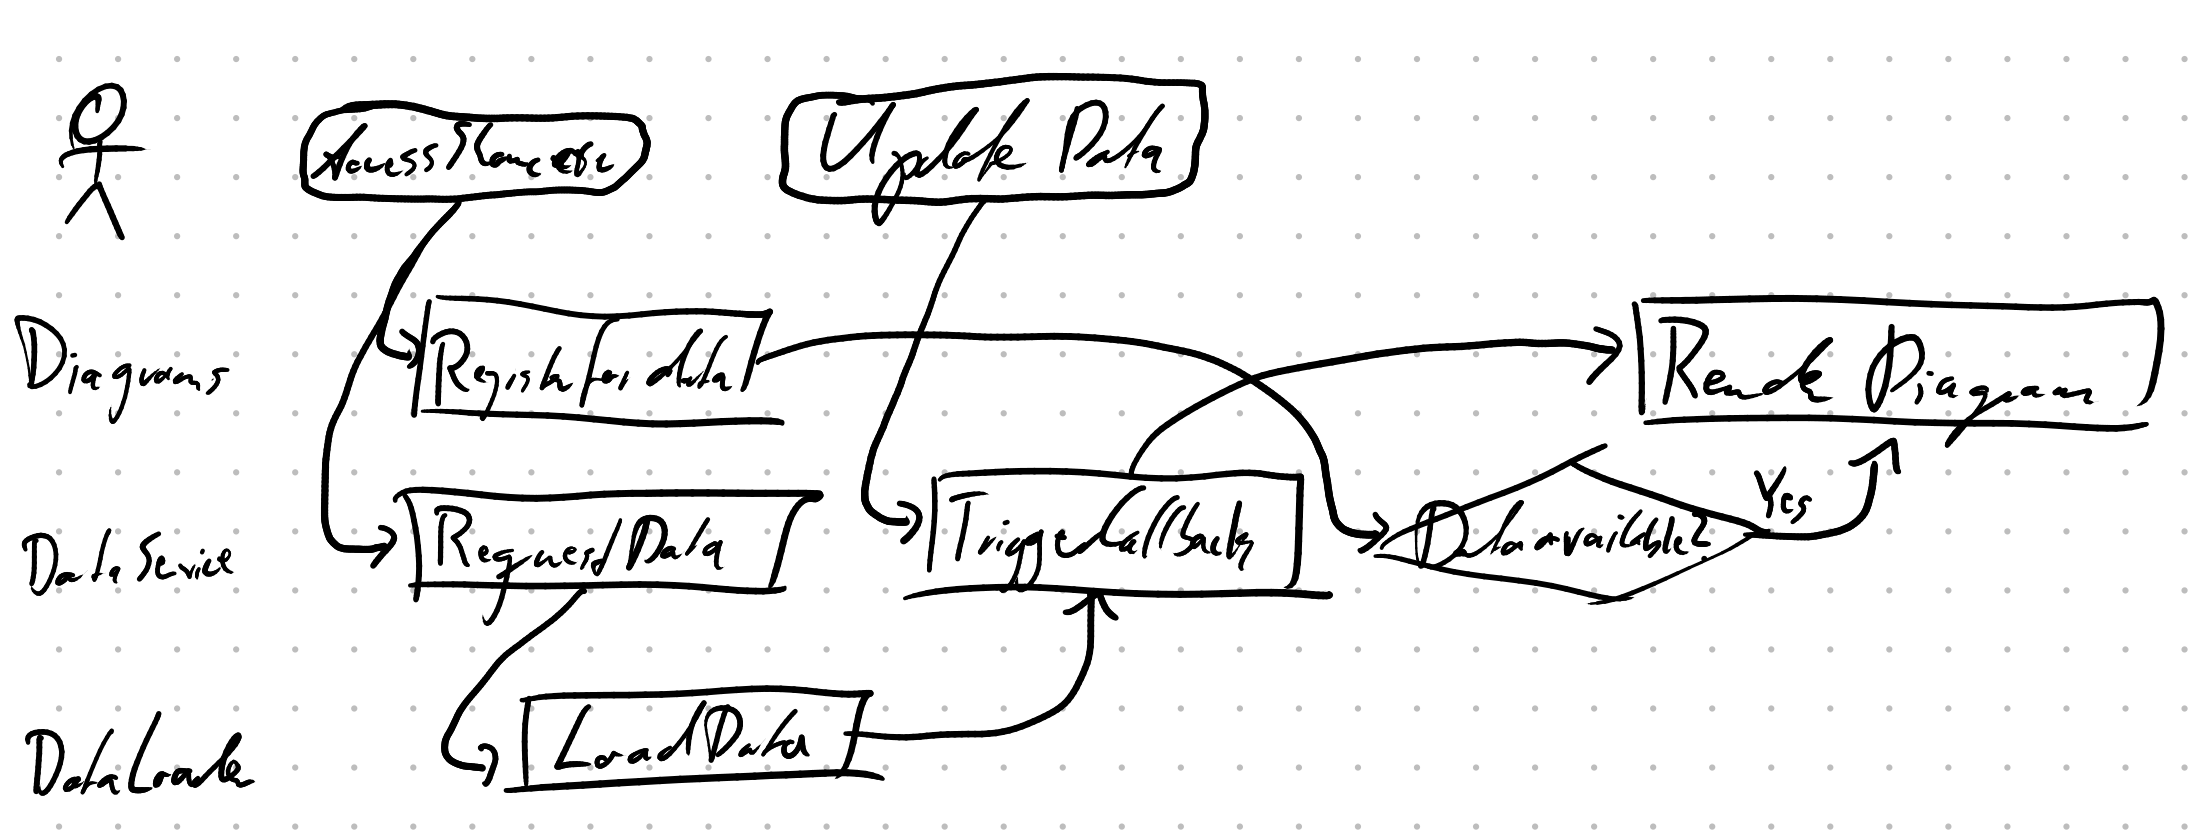
\includegraphics[width=\linewidth]{showcase-flowchart.png}
    \captionsetup{width=0.9\textwidth}
    \caption[showcase-flowchart]{This flowchart describes the behavior when loading the showcase and when data is updated. As registering with the data service and loading the data happens simultaneously, the data service returns the latest available data to the diagram when it registers for data-updates. This prevents issues which might occur due to timing.}
    \label{fig:showcase-flowchart}
\end{figure}

\begin{figure}[ht]
    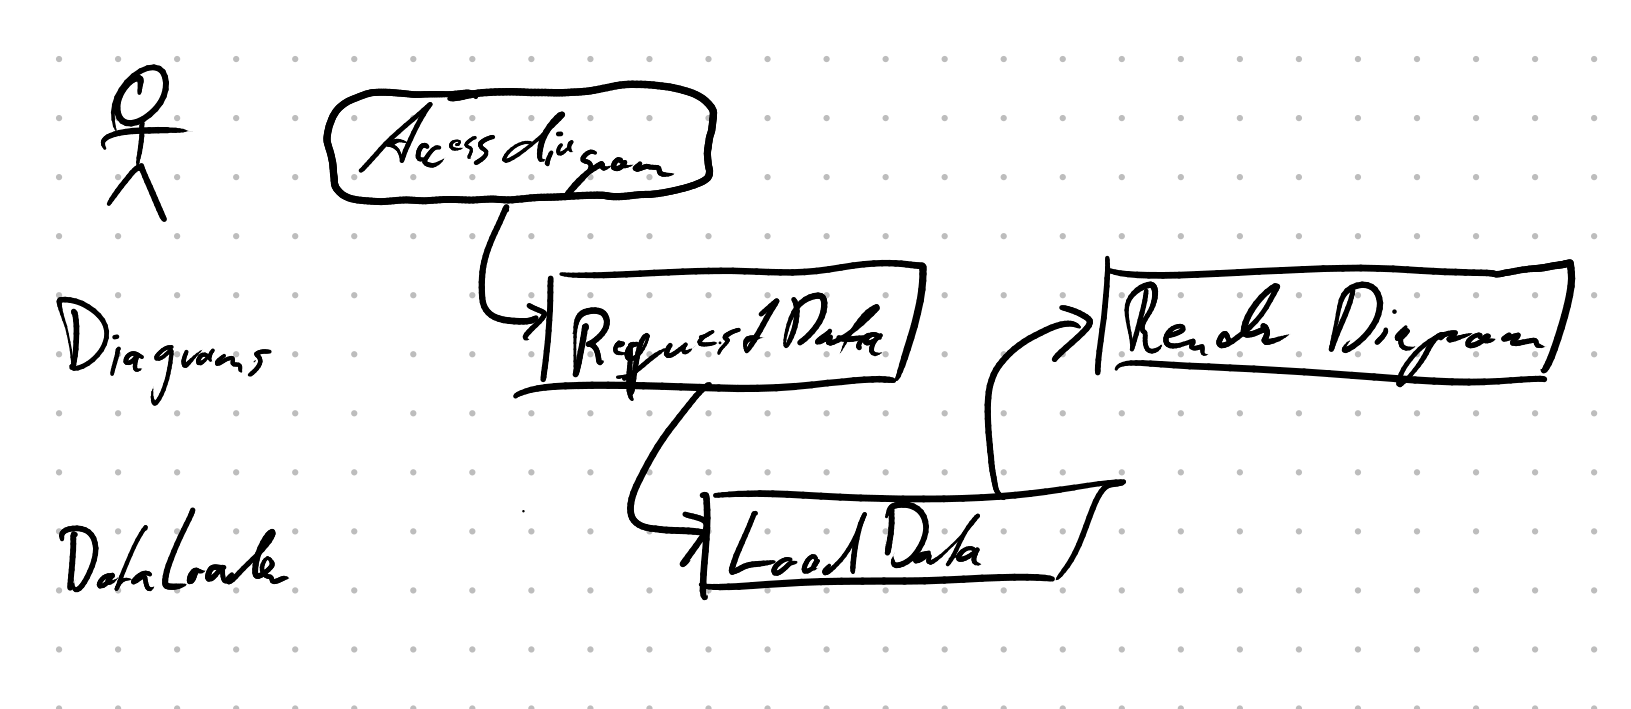
\includegraphics[width=\linewidth]{diagram-flowchart.png}
    \captionsetup{width=0.9\textwidth}
    \caption[diagram-flowchart]{This flowchart describes the behavior when loading a diagram directly. As the diagram is unable to register with a data service, it will request the data directly from the data loader.}
    \label{fig:diagram-flowchart}
\end{figure}

\subsection{Initialization}\label{sec:initialization}
All things which are independent of the data are done during the initialization of a diagram. It starts with setting some core variables. A reference to the SVG tag, which will be used as the container for the diagram, is made. It is followed by a margin definition for all four sides, where the margin of our diagram content in relation to the container size is defined. The resulting values for \verb|contentHeight| and \verb|contentWidth|, which are used as space to draw the diagram, are saved. 

Following there are a few group elements which are added to the SVG tag. Adding elements is achieved by calling \verb|.append('elementName')| on an existing element. In the first case, this element is the previously stored reference to the SVG. As the \verb|append| command returns the newly created element, it can be directly stored in a variable for later reference, or provided with attributes via method chaining. The group elements added here provide a general hierarchy for different aspects of the diagram. Listing \ref{lst:hierarchy_creation} demonstrates how this works for the bar chart. Having a proper structure in place makes working with selections easier, helps with human readability of the SVGs content and makes debugging using the browsers inspector faster. As SVG elements are drawn on top of each other depending on their hierarchical order, this can also be used to mimic layers as they would be used in drawing applications. This general hierarchy is only created to a level which is independent of the provided data and differs depending on the type of diagram. For example the bar chart has separate groups for the axes and the content, see listing \ref{lst:hierarchy_result}, while the circle diagram has groups for the background legend and the content.

\begin{minipage}{0.9\linewidth}
\begin{lstlisting}[style=htmlCSSjs, captionpos=b, caption={JavaScript code to create the hierarchy as used in the bar chart. The first line adds a new group element to the main SVG container using the \texttt{append} command. The newly added group element is saved in a constant for later references. Furthermore in line two an attribute is added to the new group element using the \texttt{attr} command and method chaining. It moves the group element from the left and top to allign with the margin definition. In each of the lines four, seven and ten, another group element is added. They are added to the previously created group element. They are all stored in constants for later reference and are provided with ID's for easier identification and debugging.}, label={lst:hierarchy_creation}]
const diagramGroup = SVG.append('g')
    .attr('transform', `translate(${margin.left},${margin.top})`);

const xAxisParentGroup = diagramGroup.append('g')
    .attr('id', 'xAxis')

const yAxisParentGroup = diagramGroup.append('g')
    .attr('id', 'yAxis')

const contentParentGroup = diagramGroup.append('g')
    .attr('id', 'content')
\end{lstlisting}
\begin{lstlisting}[style=htmlCSSjs, captionpos=b, caption={The HTML structure which results from the JavaScript code in listing \ref{lst:hierarchy_creation}. The resulting tree structure clearly separates the different aspects of the diagram. Using a hierarchical approach makes not only later selections easier, but also increases human readability and simplifies debugging.}, label={lst:hierarchy_result}]
<SVG>
    <g transform=translate(118,20)>
        <g id="xAxis"></g>
        <g id="yAxis"></g>
        <g id="content"></g>
    </g>
</SVG>
    \end{lstlisting}
\end{minipage}

If there are data independent scales, they are defined next. A common example here is a color scale for nominal values. It is used in all diagrams showing the refugees per country. When queried, it will return a new color from the provided range for each new query value. This scale does not require a predefined domain. Instead it is dynamically defined and extended with each new value querying the scale. It is important to note that when the predefined color list runs out of new colors, it starts reusing the same color list from the beginning.

\begin{minipage}{0.9\linewidth}
    \begin{lstlisting}[style=htmlCSSjs, captionpos=b, caption={Definition of the data independent color scale. \texttt{d3.schemeDarkv2} is a predefined list of color values which is  used as the range of the scale.}, label={color_scale}]
const colors = d3.scaleOrdinal(d3.schemeDark2);
    \end{lstlisting}
\end{minipage}

If there are any static elements, they are also defined in the initialization. For example the tooltip used by the tree map or the center text fields in the donut-chart. Even though the data which these fields are supposed to show is not yet known, these fields are persistent and can therefore already be created here.

Finally any general helper functions are also defined here. Both diagrams about the cumulative refugees per day make use of a date conversion function, which produces a nicely formatted date string from a JavaScript date object. The resulting strings are in the form of mmm-DD, for example Feb-07 or Jun-15.

\subsection{Render}\label{sec:render}
Following the initialization section is the render function. The render function is called once in the beginning and every time the data set changes. The render function covers all data-dependent tasks, including the implementation of the data joins and general update pattern. As the implementation of the render function greatly varies between the diagrams, all common features are described first. Afterwards the specifics for each diagram are described. If there are helper functions or constants required by the render function they are defined first. 

As all the diagrams make use of transitions for animations, a transition is defined with a duration of 1500 milliseconds. This transition is later called for each element which should be animated. Defining the transition here allows for all later calls to not only take the same amount of time without having to change the duration in more than one position, but also to reuse the same transition instance.

\subsubsection{Scales}
The data-dependent scales in this thesis are mostly used to calculate the coordinate position and sizing of elements in the diagrams. The bar chart for example defines two scales. A linear scale to find appropriate x-coordinates and a scale band for the y-coordinates of each bar. As these scales domains depend on the range of the provided data set, it is necessary that they are redefined with every render call.

\subsubsection{Data Joins}
After the scales are defined, the data joins are created. While some diagrams, like the bar chart, only use a single data join, other diagrams, like the circle graph, make use of several data joins. Usually this is in accordance to how many independent parts the diagram consists of. The circle graph uses one data join for the size legend in the background and to update the circle showing the current data as well as the text showing the current number of total refugees.

As all diagrams in this thesis can react to data changes, they have a custom identifier function. For the refugees per country data set in this thesis, the identifier function is \verb|d => {return d.country}|.

When a data join is initially created, or when data points are added, there is not a sufficient amount elements in the selection to pair them with data entries. D3 will therefore create empty placeholders for these elements. To make these placeholders become a part of the DOM, the \verb|.join()| function is added after the \texttt{data()} call. There are two ways to use the join function. One can either pass a string which will result in adding a matching tag to the DOM, or define functions for the general update pattern. When using the simple string method, the attributes and style for each new element can then be defined by method chaining. This approach is reasonable for diagrams that do not need to react to data changes. As all diagrams in this thesis implement the full extent of the general update pattern to be able to react to changing data and use the full possibilities of D3, the second approach is used.

\subsubsection{General Update Pattern}
%\textcolor{red}{
%How is this implemented? Where does it come into play?}

When the \texttt{join} function is called, instead of passing a single string as parameter, three functions can be passed as parameters. These three functions correspond to the three cases of the general update pattern and describe their respective behavior. Each of the three functions has one input parameter, corresponding to the respective sub-selection. In the enter function an element is added to the DOM. In the update function existing elements are updated to accommodate for data changes and therefore possibly removed or newly added elements as well. In the exit function elements are removed. As this is the default behavior, the exit function definition can be omitted if no extra behavior is desired. All three functions run on all the elements of the appropriate sub-selection.

The enter function adds the applicable element to the SVG. Therefore the first part of the enter function is usually an \texttt{.append(string)} call. The string describes the tag which will be added to the DOM. Afterwards the applicable styles, attributes and sub-elements are added. This can be achieved with the \texttt{.attr("attributeName", "value")}. While styles can be added with the \texttt{.style("property", "value")} function, the same can be achieved more cleanly by predefining styles in the CSS and adding applicable classes to the element. The selector used to define the current data join, should be able to match the newly created element as well. Therefore enough attributes need to be provided. This is important when the selection is recreated for updating the diagram. When positioning and sizing a new or existing element the scales are used to compute the applicable coordinate space.

The update function is necessary when the diagram should be able to react to data changes. It is usually similar to the enter function, in that it adjusts the positioning and sizing of the elements according to the possibly changes scales. 

The exit function is defined by default to simply remove the applicable elements.

All three functions can make use of animations and transitions to improve their feel. The diagrams created for this thesis only animate the enter and update behavior. Why animations are useful and how they are implemented is described in the following section.

\subsubsection{Animations}
%\textcolor{red}{
%What are they? How do they work? Why are there two kinds? What makes them tick?}

Animations can improve the feel, appeal and readability of diagrams. When a diagram is updated due to data changes, it is easier to understand and see the changes when for example bars in a bar chart shift to their new positions, instead of a seemingly entirely different diagram popping up. The animations allow the viewer to keep track of the existing entries and visually follow any changes. For example the growth or shrinking of the length of a bar in a bar chart. Animations can also be used when initially drawing the diagram, to guide viewer attention.

Animating elements in D3 is achieved by using transitions. Transitions are called from a selection and run on all the elements of the selection. A transition requires a duration and can also be provided with a delay and an easing function to improve the feel. The duration and delay are both in milliseconds. Animating numerical or color values is very easy with transitions. It is only required to call the attribute or style with the target value and the transition function will calculate and show interpolated frames. This makes it very fast and easy to animate for example positioning or sizing of elements.

Instead of using the default behaviors for numbers and colors or when trying to animate other values like SVG paths, a tween function can be defined using \verb|attrTween| or \verb|styleTween|. Both tweens need to return a function which will be invoked for each frame of the animation, with a time value between 0 and 1, depending on the frame. The returned function must itself return a value, which is applied to the desired style or attribute every frame. In this thesis custom tweens are only specifically defined to animate SVG path tags in the donut chart (see listing \ref{lst:donut-chart}).


\subsubsection{Bar Chart}
%\textcolor{red}{
%How does it work? Which d3 features does it use? how do they work?}
The bar chart, as well as the following implementations of the donut chart, the tree map and the Sankey graph all make use of the dataset containing the number of refugees per country they fled to.

The bar charts first defines two scales, the \texttt{xScale} as well as the \texttt{yScale} (see \ref{app:bar-chart} lines 42ff). The \texttt{xScale} is a linear scale to convert from a domain of the refugees [0, HighestNumberOfRefugeesInAnyCountry] to a range of the available space [0, contentWidth]. This allows to find the appropriate x-coordinate for any number of refugees. It is used to draw each bar to its appropriate length. The \texttt{yScale} converts from any given country to a y position is done using a scale band. Therefore the domain is defined by providing an array of all possible countries and the range is [0, contentHeight]. This allows the proper height positioning of each bar using the resulting y-coordinate.

The bar chart also makes use of axes. The y-axis shows the countries, while the x-axis shows the amount of refugees. D3 has predefined functions to create axes from scales. An axis in D3 consists of many ticks. By default each tick has a label and a small line indicating its position. Furthermore there is a start and end line to indicate the whole domain. The bar chart removes all the domain lines for styling reasons. The tick lines for the y-axis are also removed, as they are unnecessary here. The x-axis tick lines are extended to cover the whole diagrams height. This is done to have a proper reference to read out the bars length.

\begin{minipage}{0.9\linewidth}
    \begin{lstlisting}[style=htmlCSSjs, captionpos=b, caption={The x axis implementation of the bar chart. The first constant defines the tick format. For each number there should be two significant digits. As the zero value is represented as "0.0" to match the previous rule of two significant digits, it is simply replaced by "0". The second constant defines the function creating the axis. The previous tick format is passed here. Furthermore the \texttt{tickSize} is set to the height of the diagram. This way the initially small tick lines now cover the whole height of the diagram and allow for easier and more accurate readouts. Finally the \texttt{xAxisParentGroup} element, which is part of ther permantent hierarchical structure of the bar chart, calls the \texttt{xAxis} function. This adds the Axis to the diagram. As a last step the domain lines are selected and removed for styling reasons. (Section from \ref{app:bar-chart} lines 60ff)}, label={lst:bar-chart-axes}]
const xAxisTickFormat = number =>
    d3.format('.2s')(number)
        .replace('0.0', '0');

const xAxis = d3.axisBottom(xScale)
    .tickFormat(xAxisTickFormat)
    .tickSize(-contentHeight);

xAxisParentGroup.call(xAxis)
    .attr('transform', `translate(0,${contentHeight})`)
    .select('.domain')
        .remove();
    \end{lstlisting}
\end{minipage}

Each bar in the bar chart is composed of a \texttt{rect} for the bar itself and a \texttt{text} field as the label with the precise amount of refugees. The \texttt{rect} and \texttt{text} are both children of one group element with the \texttt{bar} class as attribute. Due to this structure, the bar chart only requires a single data join. The required selector matches all group elements with the \texttt{bar} class. In the enter sub-selection of the general update pattern, first a new group element with the \texttt{bar} class is added. Afterwards a \texttt{rect} as well as a \texttt{text} are added to the newly created group element. The \texttt{rect} is filled with the appropriate color by calling the color scale. Both elements are positioned and sized accordingly using the previously defined scales. The x-position of the text as well as the width of the rect are initialized as 0. These two values are animated using a transition, to reach their actual values. This way new bars always build themselves up from the left side. The text field usually tries to stick to the inside right side of the rect. In case where there is not enough space available to the left, as the bar is shorter than the number to show, the text is placed to the right of the rect.

Elements in the update sub-selection are resized in the width and text value if the number of refugees for this country or the range of the \texttt{xScale} changed. They might also be repositioned and resized in height, as new countries are added, or old ones removed from the data set. All resizing is done using the transition for smooth animation of the changes. Elements in the exit selection are simply removed.

\subsubsection{Donut chart}
%\textcolor{red}{
%How does it work? Which d3 features does it use? how do they work?}

As the donut chart shows the total amount of refugees in the center, this value is computed first. This is achieved using the \texttt{d3.sum(data, d => d.refugees)} function (see \ref{app:donut-chart} line 82). It creates the sum of all entries in the data, using the \texttt{refugees} field for each entry. After calculating this value, the appropriate text field is updated to contain the new number.

As each section of the donut-chart is made up of a path element, D3 provides two functions to generate pie and donut charts. The \texttt{d3.pie()} function calculates the appropriate start and end angle of each data-point (see \ref{app:donut-chart} lines 90ff). A padding angle has also been specified for some spacing between the sections of the diagram. The \texttt{d3.pie()} function returns a new object which holds a reference to our original data, additionally to the new sections information (see \ref{app:donut-chart} lines 96ff). 

The \texttt{d3.arc()} function is set up with an inner and an outer radius. Having an inner radius of zero generates a pie chart, whereas an inner radius greater than zero, like in this instance, creates a donut chart. The \texttt{d3.arc()} function which is set up here is later used in the general update pattern to generate SVG path objects from the pie pieces containing the start and end angles of each section.

As each section of the donut chart is made up of a \texttt{path} element nested inside a group element, the selector for the data join matches all group elements with the \texttt{arc} class. The data join is then created using the previously created pie object. In the enter selection of the general update pattern, the parent group element is created first and provided with the \texttt{arc} class. Afterwards a path element is added to this group element. This path element is colored according to the color scale. Drawing the actual arc piece is done in an attribute tween. This animates the donut chart to smoothly fill itself in the beginning. The implementation of this initial animation is almost same as the one seen in \ref{lst:donut-chart} for updating the arc sections. The only difference lies in the two \texttt{interpolate} functions using 0 as initial value instead of the respective \texttt{previousStartAngle} and \texttt{previousEndAngle}, as these two values are not assigned yet.

Lastly the path elements are registered to two callbacks, \texttt{mouseover} and \texttt{mouseout} using D3s \texttt{.on()} function (see \ref{app:donut-chart} lines 123 and 129). Both these events are used to show and update the appropriate text in the center of the donut chart. The effect which creates an outline around the currently hovered over path element is not linked to these events, but instead is achieved by CSS styling.

As the update behavior of the donut-chart consists only of updating the paths, it is fully described in listing \ref{lst:donut-chart}. The exit behavior removes appropriate sections.

\begin{minipage}{0.9\linewidth}
    \begin{lstlisting}[style=htmlCSSjs, captionpos=b, caption={The implementation of the arc update animations. As the core of the animation donut sections is used by the enter and the update behavior, it is defined first. The new values for start and end angle are stored on the node itself. This needs to be done to be able to reference these values again for the next update, as the previous angles will not be accessible through the pie object after regenerating it for an update. Finally the function which is called for each frame of the animation is defined and returned. This function first interpolates the start and end angle values using the passed interpolation functions and the time value. This time value is in the range of zero to one, depending on how far along the animation is. These newly interpolated angles define the start and end angle of the pie piece, which is then turned into a path element by calling the \texttt{arc} function for this pie piece. As the interpolate functions \texttt{interpolateStartAngle} and \texttt{interpolateEndAngle} differ for the enter and update behavior, they are defined in the respective sections. They are passed into the core \texttt{animate} function. (Section from \ref{app:donut-chart} lines 136ff)}, label={lst:donut-chart}]
// The core of the donut animation is defined here.
const animate = (nodes, index, d, i, j) => {
    nodes[index].previousStartAngle = d.startAngle;
    nodes[index].previousEndAngle = d.endAngle;
    
    return time => {
        d.startAngle = i(time);
        d.endAngle = j(time);
        return arc(d);
    };
};


[...].call(update => update.transition(t)
    // The update animation for the donut pieces is specified here.
    .attrTween('d', (section, index, nodes) => {
        const interpolateStartAngle = d3.interpolate(nodes[index].previousStartAngle, section.startAngle);
        const interpolateEndAngle = d3.interpolate(nodes[index].previousEndAngle, section.endAngle);

        return animate(nodes, index, section, interpolateStartAngle, interpolateEndAngle);
    }));
    \end{lstlisting}
\end{minipage}


\subsubsection{Tree map}
%\textcolor{red}{
%How does it work? Which d3 features does it use? how do they work?}
As the tree map is intended to work with hierarchical data, it requires all data points to have a link to their parent data point. There is only one data point without a link to a parent, which serves as the root element. As the refugees per country data set is not in hierarchical structure, this is simulated first. Therefore a dummy object is added to the data array. Using the \texttt{d3.stratify()} command turns the data set into a tree object by connecting each data point to a parent, in this case the dummy object (see \ref{app:tree-map} line 70). The dummy element has no parent and serves as the root of the tree object. After removing the dummy element from the data again, the sum of refugees in the tree object is calculated. Using the \texttt{d3.treemap} command and providing it with information about the available space and padding between elements provides the trees leafs with their relevant size and position information (see \ref{app:tree-map} line 85).

The general update pattern adds a \texttt{rect} for each leaf of the tree object before styling it appropriately and animating its size and position. The \texttt{mouseover}, \texttt{mousemove} and \texttt{mouseout} events are registered for showing, updating and hiding the tooltips content and position, as the mouse moves over a \texttt{rect} in the tree map. The update selection smoothly moves and resizes the rects when applicable, while the exit selection removes them.


\subsubsection{Sankey diagram}
%\textcolor{red}{
%How does it work? Which d3 features does it use? how do they work?}
The Sankey diagram consists of nodes and links. Therefore these two arrays are constructed first. Each node represents one country. The links describe the flow of values, in this case refugees, between nodes. This is achieved by providing a source node, a target node and the value. To be able to show a flow from the Ukraine to the other countries, the Ukraine is added as a node. All countries from our data are added as nodes, as well as a link to the Ukraine node is created. The resulting arrays are provided to the \texttt{d3.sankey()} function (see \ref{app:sankey} line 48). This function is not part of the default D3 namespace. Instead it is added by additionally importing the Sankey package in the Sankey diagrams HTML page header. The \texttt{d3.sankey()} function adds additional information to the nodes and links allowing for appropriate placement of the according elements. It also adds all the links' values to create a source value for the Ukraine node.

The Sankey diagram makes use of two data-joins. The first one links the nodes to appropriate group elements. During the enter behavior, each group elements is filled with a \texttt{rect} and a \texttt{text} element. The \texttt{rect} represents a node in the Sankey diagram and is sized according to the number of refugees and styled according to the country using the color scale. To make the color scale consistent with the other diagrams, the Ukraine node is provided with a fixed color. This prevents the Ukraine node from querying the color scale and creating inconsistency with the other diagrams which do not contain a representation for the Ukraine. The \texttt{text} label contains the name and amount of refugees per country. It is placed next to the appropriate \texttt{rect}s. This can be on the left or rights side, depending on the x position of the rects. If the rect is in the left half of the diagram the label is right, if the rect is in the right half the label is left. Both rect and text make use of transitions to smoothly build up the diagram. The text also makes use of a small delay to the transition by using the \texttt{.delay(100)} function (see \ref{app:sankey} line 93).

The second data join takes care of the links. They are matched to path elements. Each path is styled to match with the country it leads to. The required SVG path is created using the \texttt{d3.sankeyLinkHorizontal()} command (see \ref{app:sankey} line 111). As the resulting path is only a single line, the \texttt{stroke-width} attribute corresponds to the size of the link. The links are also animated using the transition. When initially appearing, the links are provided with a delay before fading into existence after the nodes have settled in their positions. The update behavior makes sure that the links are smoothly transitioned to their necessarily position and the width adjusted as needed.

\subsubsection{Circle graph}
%\textcolor{red}{
%How does it work? Which d3 features does it use? how do they work?}
The circle graph, as well as the area graph described in the following section both make use of the data set about the cumulative refugees per day.

The circle graph makes use of two data dependent scales. A time scale is created using \texttt{d3.scaleQuantize()} (see \ref{app:circle-graph} line 55). It is used for converting the time slider value to an actual date. As the time slider value provides a value between zero and one, this domain is mapped to the range of available dates in the data set. The second scale is used to get the correct radius of the circle. Because the area of the circle corresponds to the number of refugees, it is important to not scale the radius linearly. This would lead to circle areas which do not represent the correct number of refugees. Scaling the radius linearly would introduce a lie-factor higher than one. In fact, due to the relation between a linear change in radius and a change which keeps the area consistent, the lie factor increases, the higher the amount of refugees is. To avoid this, a \texttt{d3.scaleSqrt()} is used (see \ref{app:circle-graph} line 60). The domain is set to [0, HighestNumberOfTotalRefugees] and the range to [0, contentHeight/2]. This scale is also used for drawing the background legend. This is achieved by getting the ticks of the scale and saving the appropriate values in an array. This array is rendered in circles using the first data-join. This data-join draws and updates a circle and a text label for each tick.

As the actual content of the diagram does not draw one mark per data-point, as the refugee number for only one data entry is shown at a time. The time scale is used to determine which is the currently selected date from the time value which is provided by the slider in the range of zero to one. The resulting date is used to get the corresponding data for that date from the data set. This allows the diagram to reuse only use one circle and one text label in its representation. Therefore the second data join also looks a bit different. Instead of linking actual data, an array with an arbitrary single entry is linked to the selection. Without this single element, D3 would not draw the circle, as it assumes that there is no data to show. The identifier function also always returns the same value, no matter what data was linked. This makes sure that the same circle element is matched by the selector on each render call, as to not draw a new circle every time the diagram is supposed to update. The circle and text are both created and styled using the data which was found for the current date.

\subsubsection{Area graph}
%\textcolor{red}{
%How does it work? Which d3 features does it use? how do they work?}

The area graph makes use of the same time scale as the circle graph. Additionally it uses a linear scale for the y-axis and a scale band for the x-axis. The y-axis represents the number of refugees, while the x-axis shows the days. Both axes are added to the diagram in the same way as is done in the bar chart. As showing all days on the x-axis would be too dense, the values are filtered and only 15 equidistant days are shown. This is achieved by using JavaScript \texttt{filter} function for arrays and specifying a custom filter which is to be evaluated for each entry in the domain of the x-axis scale band (see \ref{app:area-graph} line XX).

The main content of the area graph consists of two parts. One part shows the area, while the other one is the date line showing the current date. The area and the line following along the top of the area, the top-line, are two separate path elements. Their definition can be seen in listing \ref{lst:line-area}. Because the area and line both cover the whole range of data at once, the data join, which creates and updates them, uses the same single element dummy data as the circle graph. When creating or updating the line and area, the whole data set is passed to the respective functions.

\begin{minipage}{0.9\linewidth}
    \begin{lstlisting}[style=htmlCSSjs, captionpos=b, caption={The first constant defines the function for creating the top-line of the area graph. This is achieved by specifying functions for x and y values. D3 uses them to calculate the position of each point on the line. Using the arrow functions here applies this for each entry of the data set which is passed as a parameter when calling this function. When the function is called and a data set is provided, by calling \texttt{line(data)}, the line is constructed by calculating the according x- and y-positions for every data point. Defining and creating the area works in similar fashion. Yet there are two y-positions for each x-position. \texttt{y0} is the bottom of the shape, while \texttt{y1} is the top. Switching the definition of \texttt{y0} and \texttt{y1} results in a reversed direction of the SVG path describing the outline of the shape. The \texttt{d3.area()} function allows for a huge variety of shapes. Yet it is not possible to create concave ends on the right or left side of the shape, assuming left and rigth are oriented horizontally. Of course the created shape can be rotated and oriented using all possible SVG tags and attributes. (Section from \ref{app:area-graph} lines 111ff)}, label={lst:line-area}]
const line = d3.line()
    .x(d => xScaleWithOffset(d.date))
    .y(d => yScale(d.refugees));

const area = d3.area()
    .x(d => xScaleWithOffset(d.date))
    .y1(contentHeight)
    .y0(d => yScale(d.refugees));
    \end{lstlisting}
\end{minipage}

The date line is made up of three elements. A circle element rides on the top line of the area, a vertical line to indicate the current day on the x-axis and a text label to show the days refugee value. All three parts are simply created and updated in the second data-join. This data-join makes use of the same kind of dummy data as seen in the previous data-join and the circle graph.


\section{Showcase} \label{sec:showcase}
%\textcolor{red}{
%How is the showcase structured? How can you get there? Why does it exist? Who might benefit? How can you reuse a part the interesting parts?}

To bring all the diagrams together, a showcase has been created. It  is split into two main parts. Firstly, all the diagrams showing the  refugees per country they fled to, are shown. Secondly, the diagrams for refugees over time are shown. As all diagrams in one section represent the same data set it allows for an easy visual comparison.

The showcase loads each of the diagrams into a separate \texttt{iframe} tag with a consistent aspect ratio. As the diagrams are set up to use all available space in the provided container, the showcase makes sure to size the \texttt{iframe} containers appropriately. When a diagram is loaded in the showcase, it also registers with the applicable data service. This allows the data service to update the diagram as the data is changed, as is described in the following section.

\subsection{Data Updates}
%\textcolor{red}{
%How can you simulate data changes? Why is this useful?}

Each section of the showcase has a table which allows for data manipulation. Rows of data can be modified, added or removed here. The data changes here are not persistent and are therefore not saved in the original data files. While the correctness of the initial data is not guaranteed, arbitrarily changing the data entries obviously falsifies the shown data. Changes in the data are registered by the respective data service. It created a new data set from the data in the table when updating. This new data set is passed long as a parameter to all the applicable diagrams when calling their render function to update.

For this thesis it is important to be able to modify the data, as one of the core features of D3 tested in this thesis is reacting to changes in data. This manual style of modifying data is probably not so common in real world applications. Yet it is easy to replace these manual data changes to regular API calls or other automatically updating data sources. As the source of the data changes does not matter for the functionality of D3, the manual approach chosen here is sufficient in demonstrating the possibilities of D3.

    \chapter{Discussion}\label{sec:discussion}
The discussion evaluates the results of this thesis. Therefore it is split into two parts. The first part, section \ref{sec:diagrams-dis}, is about the diagrams and comparing them to each other. Section \ref{sec:d3-dis} contains the second part of the discussion and tries to answer the initial questions about the potential of D3 in data visualization.

\section{Diagrams}\label{sec:diagrams-dis}
The first four diagrams show the data about the refugees by country crossed into. While the underlying data is the same, the resulting diagrams are quite different. 
The donut chart and tree map make it immediately obvious, that almost half of all refugees went to Poland. While this is hard to guess from the bar chart without a ruler or calculator, the vertical spacing of the nodes in the Sankey diagram also does not make this obvious.
Only the donut chart and the Sankey diagram allow the viewer to immediately see the total amount of refugees. While the bar chart and tree map also contain this information, they would require the viewer to calculate it themselves, defeating the purpose of data visualization.
The Sankey diagram and bar chart directly show all the numbers of refugees per country. This information can be found in the donut chart and tree map as well, but only by using the mouse to inspect the diagrams more closely. This can be a struggle when trying to get more precise data about the refugees which went to Belarus, as their amount is so small, that these two diagrams hardly show Belarus at all.
While the shown legend is universally true, both the Sankey diagram and the bar chart also directly show the names of the countries, making comprehension of the data more easy.
The Sankey diagram is also the only diagram which conveys the flow from the Ukraine to the other countries. The other diagrams only achieve this through context, not in their actual graphic.

When data is updated, all four diagrams smoothly transition to their new states. This makes the changes quite easy to follow and pleasant to look at. The tree map can sometimes be a bit confusing, as the different rectangles can shift across each other.

The two diagrams showing the cumulative refugees per day, are quite different from each other. While the circle graph actually only ever shows the value for a single day, the area graph shows the whole extend of the data with an extra indicator for the current day.
Due to the scaling of the radius in the circle diagram it can also be quite hard to read the number of refugees from the legend, especially for smaller values.
The area graph does a much better job of not only consistently showing not the number of refugees on the selected day, but also the development of the refugee count over time. Therefore it struggles with accurately showing the current date. This is easier in the circle chart, as it is simply displayed at the bottom.

When data is updated, the circle graph can be completely unaffected. Only when the data for the currently selected day is changed, or the size legend adjusts itself changes can be seen. Because of the way that the functions used to create the line and area of the area graph work, the updates of the area graph are only easy to follow when values are adjusted. When days are added and removed, it is hard to follow changes.


\section{D3}\label{sec:d3-dis}
The tree initial questions presented which this thesis tries to answer were: What is the potential of D3 in data visualization? What are the advantages and disadvantages of using D3? When should D3 be used? All three of these questions will be evaluated and discussed separately in the following discussion, beginning with the question of what D3s potential is. 

Looking at the created showcase, D3 can obviously be used to create many different types of diagrams. Looking at the examples found online, D3 has their own showcase of projects, makes this even more apparent. From simple bar and pie charts, over visualizing hierarchical data using tree maps or Sankey diagrams, like the ones created for this thesis, all the way to map based diagrams using various projections\cite{davies}, physics enabled bubble graphs\cite{carter_2012} and pseudo 3D animations\cite{davies_sphere}. Of course D3 can also be used to created animations which do not necessarily serve data visualization purposes, like the tadpoles example\cite{bostock_2020}. Due to D3's low level approach, fast speed, and the general update pattern, D3 can be used to create all visualizations one can imagine and have them react to data changes in real time. As D3 is built around simple DOM manipulation, it can also be used for other use cases. One can create HTML tables and populate them with data. One can make small animations to add visually appealing aspects to a website. Or maybe one can adapt the scales for their own needs of converting data. But what are the advantages an disadvantages of D3?

When working in a web environment, it is always easy to start using D3 as well. Its independence from any framework and its pure JavaScript implementation, make it possible to include D3 in any web-based project. On the other hand, if one is not already working on a web-based project but still wants to use D3, one has to deal with all the additional overhead of working with a web technology stack. Whilst importing the D3 library is really easy, the initial learning curve is everything but easy. Without first internalizing the core concepts of D3 and SVG, it is impossible to make any kind of visualization. While this is true for any framework or technology, the concept of the data joins and the general update pattern seem especially abstract. Yet it is crucial to understand it when a diagram is supposed to react to data changes.
While learning the basics of D3 is quite a big hurdle, it can be broken down by first creating only static diagrams. This can be achieved without a deeper understanding of the general update pattern. While D3s low-level approach is cumbersome to comprehend initially, it actually allows D3 to be very flexible.
In addition, while there are a lot of examples and tutorials, they are often too complex to understand as a beginner, or use varying versions of D3 or JavaScript styles. Besides some functionalities of D3 being obsolete in newer versions, the different styles of JavaScript can be additionally confusing when the developer is not familiar with the evolution of JavaScript.
Once one understands how D3 works, it can be quite fast to create basic diagrams. Once one properly understands the general update pattern and selections, it is also not too difficult to react to data changes. Yet trying to animate diagrams can become tricky. It depends on the elements which are used and which attributes need to be animated. As all elements have to be manually specified, one has full control over the appearance and behavior of the diagrams. This allows D3 to adapt to any existing style guides, yet is also very time consuming. It also allows creating diagrams with a high lie-factor or a bad data-ink ratio. This risk can be mitigated using a more high-level library. High-level libraries also allow for the automatic creation of legends, instead of having to create them manually as was done in this thesis.

Another concern might be the performance of D3 when dealing with many marks in a diagram. Therefore the limits of smooth animation of the bar-chart and the tadpoles example\cite{bostock_2020} were briefly tested. Of course these results vary from device to device. In this case, it was possible to smoothly animate up to approximately 1200-1300 tadpoles. The bar-chart is harder to evaluate. The singular bars approach, and partially pass, the limits of a singular pixel in thickness, and therefore their visibility on the screen, with this number of entries in the diagram. While this thesis does not provide a proper performance test and comparison with other visualization libraries performances, it can be safely assumed that performance will not be an issue for most diagrams.

So when should one use D3? This depends on the task at hand. If the goal is to create some diagrams as a one time job, D3 is unnecessarily complex. Tools like Excel can easily excel here. Even when working with a web project, D3 is probably too complex. Most developers will find all necessarily functionality using libraries like Chart.js\cite{chartjs} or the Plotly\cite{plotly} JavaScript library, which is actually built on top of D3 to offer a more high level approach to data visualization. Both these open-source libraries allow creating some of the most common diagrams without having to learn all the quirks of D3.
Yet if someone is to create a custom visualization or wants more fine control over all aspects of a diagram, D3 can handle it.
Nevertheless, due to the high initial learning curve getting into D3 can only be recommended when the creating custom visualizations, which high level libraries can not provide.

    \chapter{Conclusion}\label{sec:conclusion}
%\textcolor{red}{
%How well did it work? Was it worth the effort? What could be improved?}

While D3 is an immensely powerful tool, learning and understanding the core concepts of D3 took a surprisingly long time. While there are many examples, the inconsistencies in D3 versions as well as JavaScript versions were quite confusing. Having never worked with D3 and only having very limited experience with JavaScript, it took a fairly long time to get used to both.
Even now, if I was tasked to create some simple diagrams, I would probably use a more high-level library. Unless the required diagrams require the full potential of D3.
A few parts have been especially cumbersome. While animating updates with transitions is usually easy, creating a smooth animation for the donut chart took longer than expected. Having to work with the custom attribute tweens and storing information on the DOM element itself, made this even more confusing. Yet this was in part due to my lacking proficiency in working with JavaScript and the differences between function declarations using arrow functions and the function keyword. I was also unable to animate the area graph in a way where the date line follows the line along the top of the area. Furthermore it would be nice if the date line would be draggable using the mouse. This is something which can most certainly be done. But not by me in the time span of creating this thesis. Creating the right selections and sub-selections when implementing the general update pattern also is not always easy. While drawing a diagram initially is usually an easily achievable feat, making sure that update behavior reuses existing elements is sometimes tricky. The widespread use of D3 at least helped finding information on common issues, which was very helpful for bug fixing.

While the implementation doesn't differ for using discrete and continuous data, it would still have been nice to show this in an actual example. Another interesting aspect which is not explored by this thesis, is working with maps and projections. A map could also have easily shown the refugee streams.

Due to the currentness of the data, the UNHCR was updating their situation page as well. On of the effects of this was that the terminology they used changed from initially mentioning refugees, to later solely mentioning border crossings. This can actually still be seen when looking at the raw data JSON file, which contains the cumulative number of refugees per day. It contains a description clearly mentioning the data being about refugees. As the diagrams and showcase were implemented before writing the text for this thesis, the renaming was glossed over, as all the created work would have to be redone. This is also why the code files always mention refugees. 

Finally, while it was interesting to work with D3 and get to know its immense potential, it is devastating to see that, yet again, millions of people have been displaced by unnecessary violence and aggression.

    %\chapter{Sources}
This should ideally done automatically by bibtex.
    
    \bibliographystyle{IEEEtran}
    \bibliography{sources}
    
    \appendix
\chapter{Appendix}

\section{Bar Chart - JavaScript}
\lstinputlisting[style=htmlcssjs,label=app:bar-chart]{../project/diagrams/total_per_country/bar-chart/diagram.js}

\section{Donut Chart - JavaScript}
\lstinputlisting[style=htmlcssjs,label=app:donut-chart]{../project/diagrams/total_per_country/donut-chart/diagram.js}

\section{Tree Map - JavaScript}
\lstinputlisting[style=htmlcssjs,label=app:tree-map]{../project/diagrams/total_per_country/tree-map/diagram.js}

\section{Sankey Graph - JavaScript}
\lstinputlisting[style=htmlcssjs,label=app:sankey]{../project/diagrams/total_per_country/sankey/diagram.js}

\section{Circle Graph - JavaScript}
\lstinputlisting[style=htmlcssjs,label=app:circle-graph]{../project/diagrams/total_per_day/circle/diagram.js}

\section{Area Graph - JavaScript}
\lstinputlisting[style=htmlcssjs,label=app:area-graph]{../project/diagrams/total_per_day/area/diagram.js}
\end{document}